% Written by Daina Chiba (daina.chiba@gmail.com).
% It was mostly copied from two poster style files:
% beamerthemeI6pd2.sty written by
%	 	Philippe Dreuw <dreuw@cs.rwth-aachen.de> and 
% 		Thomas Deselaers <deselaers@cs.rwth-aachen.de>
% and beamerthemeconfposter.sty written by
%     Nathaniel Johnston (nathaniel@nathanieljohnston.com)
%		http://www.nathanieljohnston.com/2009/08/latex-poster-template/
\documentclass[final]{beamer}
\usepackage[orientation=landscape,size=a0,scale=1.2,debug]{beamerposter}
\mode<presentation>{\usetheme{OpenNMT}}
\usepackage[english]{babel}
\usepackage[latin1]{inputenc}
\usepackage[T1]{fontenc}
\usepackage{amsmath,amsthm, amssymb, latexsym}

\usepackage{array,booktabs,tabularx}
\newcolumntype{Z}{>{\centering\arraybackslash}X} % centered tabularx columns

% comment
\newcommand{\comment}[1]{}

% (relative) path to the figures
\graphicspath{{figs/}}

\newlength{\columnheight}
\setlength{\columnheight}{105cm}
\newlength{\sepwid}
\newlength{\onecolwid}
\newlength{\twocolwid}
\newlength{\threecolwid}
\setlength{\sepwid}{0.024\paperwidth}
\setlength{\onecolwid}{0.24\paperwidth}
\setlength{\twocolwid}{0.4\paperwidth}
\setlength{\threecolwid}{0.19\paperwidth}

\title{\huge OpenNMT: Open-Source Toolkit for Neural Machine Translation}
\author{Guillaume Klein$^\dagger$, Yoon Kim$^*$, Yuntian Deng$^*$, Jean Senellart$^\dagger$, Alexander M. Rush$^*$}
\institute[]{Harvard University$^*$, SYSTRAN $^\dagger$}
\def\conference{2017 Annual Meeting of the Association for Computational Linguistics}
\def\yourEmail{opennmt.net}

\begin{document}
\begin{frame}[t]
  \begin{columns}[t]
    \begin{column}{\onecolwid}

      \vskip3ex

      \begin{block}{Technologies}
        {\bf OpenNMT is an ecosystem based on multiple technologies and frameworks:}
        \vskip1ex
        \begin{itemize}
        \item \alert{OpenNMT}: the original full-featured project in \emph{LuaTorch}, focusing on maintainability, user support, and production.
        \item \alert{OpenNMT-py}: a \emph{PyTorch} clone of OpenNMT, focusing on research and modularity.
        \item \alert{CTranslate}: an inference engine for OpenNMT models in C++ and \emph{Eigen}, focusing on embedded and production environments.
        \end{itemize}
      \end{block}

      \vskip3ex

      \begin{block}{Features}
        {\bf OpenNMT implements many additional features on top of the baseline model:}

        \vskip1ex

        \begin{itemize}
        \item factored translation for richer text representation;
        \item tokenization and data preparation tools;
        \item model variants: bidirectional encoder, convolutional encoder, variational dropout, etc.;
        \item learning rate decay strategies;
        \item advanced model retraining and adaptation;
        \item beam search normalization;
        \item \ldots~and many more!
        \end{itemize}

      \end{block}

      \vskip3ex

      \begin{block}{Tasks}
        {\bf OpenNMT supports other tasks than machine translation:}

        \vskip1ex

        \begin{itemize}
        \item Sequence tagging.
        \item Language modeling.
        \item Speech-to-text, using a pyramidal RNN encoder.
        \item Image-to-text, using a combination of CNN and RNN layers.
        \end{itemize}

        \vskip2ex

        For example, \emph{Im2Text} (\alert{github.com/OpenNMT/Im2Text}) is an extension that can be used for image captioning, optical character recognition, or \LaTeX~decompilation:

        \vskip2ex

        \begin{figure}
          \begin{center}
            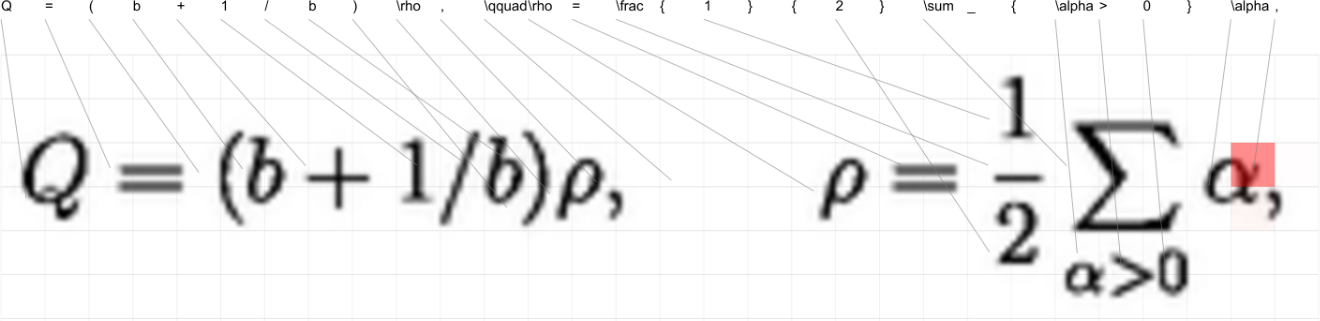
\includegraphics[width=0.8\onecolwid]{im2text}
          \end{center}
        \end{figure}

      \end{block}

    \end{column}

    \begin{column}{\twocolwid}
      \vskip3ex

      \begin{figure}
        \begin{center}
          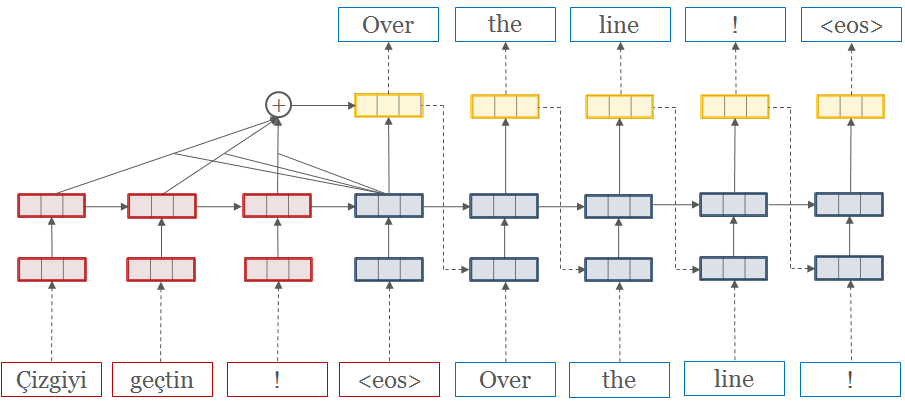
\includegraphics[width=\twocolwid]{seq2seq}
          \caption{The standard sequence-to-sequence model.}
        \end{center}
      \end{figure}

      \vskip3ex

      \begin{alertblock}{}
        \baselineskip=.7\baselineskip
        \vskip1ex
        {\bf OpenNMT is an industrial-strength and open-source neural machine translation ecosystem featuring:}
        \vskip1ex
        \begin{itemize}
        \item Ready-to-use and highly configurable implementations in \emph{Torch} and \emph{PyTorch}.
        \item State-of-the-art translation accuracy and competitive training efficiency.
        \item Extensive set of model and training options covering a large set of needs of academia and industry.
        \item Extensions to allow other sequence generation tasks such as summarization, image-to-text, and speech-to-text.
        \item Standalone and dependency-free inference engine in C++.
        \end{itemize}
        \vskip1ex
      \end{alertblock}

      \vskip3ex

      \begin{columns}[t,totalwidth=\twocolwid]
        \begin{column}{\threecolwid}
          \begin{block}{Neural Machine Translation}

            Neural machine translation (NMT) is a new methodology for machine translation that has led to remarkable improvements, particularly in terms of human evaluation, compared to rule-based and statistical machine translation (SMT) systems.

            \vskip2ex

            OpenNMT implements the attention-based encoder-decoder architecture that models the probability of a target sentence $w_{1:T}$ given a source sentence $x_{1:S}$ as:

            \begin{align*}
              p(w_{1:T}| x) = \prod_{1}^T p(w_t| w_{1:t-1}, x; \theta)
            \end{align*}

            \vskip2ex

            This modeling is usually achieved using LSTM recurrent networks which allows long term dependency learning.
          \end{block}
        \end{column}

        \begin{column}{\threecolwid}
          \begin{block}{State-of-the-art system}
            OpenNMT implements models and training procedures that achieve competitive results in system comparison, e.g. in the recent WMT 2017 translation task:

            \vskip2ex

            \begin{table}
              \begin{tabular}{l r}
                {\bf System} & {\bf BLEU-cased} \\
                \midrule
                uedin-nmt-ensemble & 28.3 \\
                LMU-nmt-reranked-wmt17-en-de & 27.1 \\
                {\bf SYSTRAN-single} & {\bf 26.7} \\
                \bottomrule
              \end{tabular}
              \vskip1ex
              \caption{Top 3 on English-German \emph{newstest2017}.}
            \end{table}

            \vskip2ex

            More generally, OpenNMT produces strong baselines with optimized training time and memory requirements.
          \end{block}
        \end{column}
      \end{columns}

    \end{column}

    \begin{column}{\onecolwid}

      \vskip3ex

      \begin{block}{Additional resources}
        {\bf OpenNMT provides additional resources including:}
        \vskip1ex

        \begin{itemize}
        \item A complete documentation portal (\alert{opennmt.net/OpenNMT}) for beginners to advanced users describing data preparation, models, training strategies, command line options, etc.
        \item Visualization tools for debugging or understanding.

        \begin{figure}
          \begin{center}
            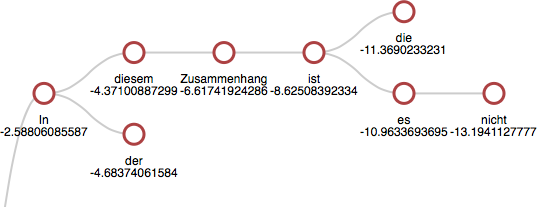
\includegraphics[width=0.5\onecolwid]{beam_search}
            \caption{Beam search visualization}
          \end{center}
        \end{figure}
        \end{itemize}

      \end{block}

      \vskip3ex

      \begin{block}{Community}
        \begin{figure}
          \begin{center}
            
\includegraphics[width=0.5\onecolwid]{stars}
            \caption{GitHub statistics}
          \end{center}
        \end{figure}

        OpenNMT is also a community around machine translation and language modeling. The forum (\alert{forum.opennmt.net}) counts more than 200 users with daily questions on how to improve or adapt their system and training procedure.
      \end{block}

      \begin{block}{Production environment}
        \begin{figure}
          \begin{center}
            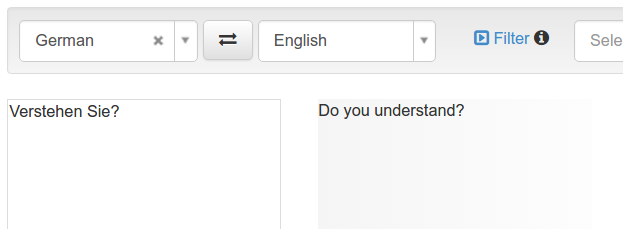
\includegraphics[width=0.5\onecolwid]{demo}
            \caption{Live demo of OpenNMT}
          \end{center}
        \end{figure}

        OpenNMT has proved to be adapted to production settings. SYSTRAN---a major translation services provider---is using OpenNMT for its Pure Neural\texttrademark~Machine Translation offering which enables higher translation quality in existing services.
      \end{block}

    \end{column}
  \end{columns}

\end{frame}
\end{document}
